\chapter{Compiling and Linking}

The feed handler will be compiled as both a standalone executable and a shared library that can
be loaded into q. Different steps and build artefacts are required for each type of binary and
can also differ based on the platform that you are compiling on (i.e. Windows or Linux). For
most of the networking code in this example, the document assumes a Windows platform with the
use of WinSock2. The rest of the code in the documentation should however be portable across
both platforms.

The "k.h" header file is available from the code.kx.com subversion repository \footnote{http://code.kx.com/svn/}.
This file defines the C API that will be used regardless of the platform and type of application you are
compiling for. The header file is compatible with both version \textbf{2.x} and \textbf{3.x} of kdb+. It is important
that you define \verb|KXVER| to be set to the correct value for the version of kdb+ you are using. The header file will
also force a compilation error if this has not been defined. You can define this in your C/C++ code as demonstrated below:

\begin{figure}[h]
\begin{lstlisting}[language=C]
#include <stdlib.h>
#include <stdio.h>

#define KXVER 3 // declaring that we want to work with v3.x of kdb+
#include "k.h"

int main(void)
{
	return EXIT_SUCCESS;
}
\end{lstlisting}
\caption{Importing the "k.h" header and defining KXVER}
\end{figure}

It is usually possible to define this from your toolchain when compiling, for example on Linux
with GCC, we could use the \textbf{-D} flag to specify \verb|KXVER| in order to define the same value at compile
time:

\begin{figure}[h]
\begin{lstlisting}
gcc example.c -DKXVER=3 -fpic -shared -std=gnu99 -o example.so
\end{lstlisting}
\caption{Defining KXVER from the command line with GCC}
\end{figure}

\section{Linux}

\subsection{Shared Objects}
On Linux, creating a shared object is simple. You just need to compile your code with the \textbf{-fpic}
and \textbf{-shared} flags. This \textbf{-fpic} flag makes the code position independent and this is
important as code included in libraries should be able to be moved \& reloaded anywhere in memory. The
\textbf{-shared} flag tells the compile to output a shared object rather than look for an entry point
in the program. The examples in the document will assume that the \textbf{-std=gnu99} flag has been passed to
the compiler also for some quality of life improvements (e.g. the ability to declare variables in for
loops).

\begin{lstlisting}
gcc example.c -fpic -shared -std=gnu99 -o example.so
\end{lstlisting}

\subsection{Standalone Executable}

Creating a standalone executable requires you to link against the appropriate object file that
contains the implementations of the functions declared in the "k.h" header. The c.o file contains
the implementations on Linux and it can be found in the \textbf{l32} and \textbf{l64} folders of the Kx
subversion repository\footnote{http://code.kx.com/svn/kx/kdb+/c/c/}.
 
 You don't need to link against this object with the shared object as the functions are already
 defined within the kdb+ process that the shared library will be loaded into. Your code for a
 standalone executable will also require an entry point (i.e. a standard definition of \textit{main}).
 
 \begin{lstlisting}
 gcc example.c c.o -std=gnu99 -o example.so
 \end{lstlisting}
 
 \section{Windows}
 
 \subsection{Standalone Executable}
 
 On Windows you will need to get the latest c.obj files from http://code.kx.com/svn/kx/kdb+/
 in either the \textbf{w32} or \textbf{w64} folders depending on whether you want to create a 32 bit or 64 bit
 process. You will also need to compile against the Winsock2 library if running as a standalone executable as this is required by the implementations.
 
 If you have a Visual Studio project set up and do not want to attempt compiling from the
 command line then you just need to drop the object into the path where Visual Studio can
 find it. The easiest way to do this is to click on \textit{"Resource Files -> Add... -> Existing Item"}
 from your solution explorer.
 
 \begin{figure}[h]
	 \centering
	 \fbox{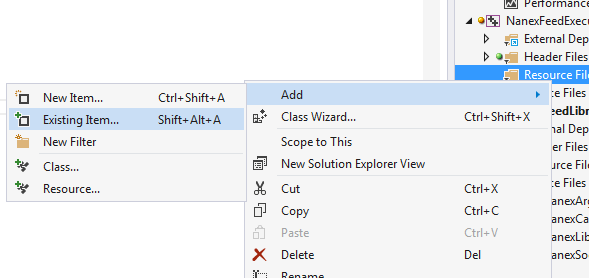
\includegraphics[scale=0.50]{figures/windows_vs2012_static_linking_alt.png}}
	 \caption{Adding an item as a Resource File via the Solution Explorer}
	 \label{addingvsresource}
 \end{figure}
 
 Another way to make sure the objects are included by the linker is to add them to the "Input"
 section of your projects resource page.
 
  \begin{figure}[h]
  	\centering
  	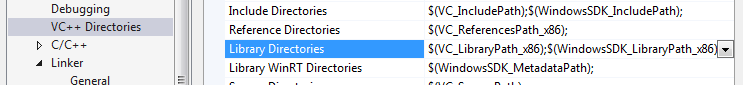
\includegraphics[scale=0.50]{figures/windows_vs2012_static_linking_dirs.png}
  	\caption{Adding an item as a Resource via the Input Resource Page}
  	\label{usingtheinputresourcepage}
  \end{figure}
 
 Note that we add \textbf{WS2\_32.lib} to input section of this page to make sure that the Winsock2 library is included. This file is included on the system path of any recent Windows installation (i.e. Windows XP or greater). Once the object files are visible to Visual Studio, you should be able to compile any code without issues.
 
 It is also possible to compile the code from the command line on Windows using \textbf{cl.exe}. This can be found by navigating to your Visual Studio installation
 location:
 
 \begin{lstlisting}
 C:\Program Files (x86)\Microsoft Visual Studio\12.0\VC\bin.
 \end{lstlisting}
 
 This folder should be added to your system PATH, or you can run \textit{vcvars32.bat} from that folder in order to make it visible temporarily from the current session.
 
 Examples of using cl.exe to compile code as a standalone executable can be found at: 
 \url{http://code.kx.com/svn/kx/kdb+/c/c/c.c}
 
 \subsection{Dynamically Linked Library (DLL)}
 
 In order to build shared objects on Windows, you will need to link against the \textbf{q.lib} file which provides the declarations of the exported objects. This is required on Windows, otherwise the functions that are defined in "k.h" will fail to link properly and the DLL file will not load into the q processes. Adding the q.lib file to your project is performed in the same way that you would add the c.obj file. You will also need to make sure you are still linking against the \textbf{ws2\_32.lib} file. One issue that may arise at runtime is crashing or inconsistent behaviour due to thread local storage (TLS). In cases where your application is incompatible TLS, an alternate implementation of c.obj called \textbf{cst.obj} is provided which should solve any issues.
 
 With the Visual Studio toolchain, the functions that are defined are not exported into your library
 by default. You will need to explicitly list the functions that are to be made available in your
 library by creating a \textbf{.def} file or by using the \verb|__declspec| keywords. The simplest .def file that
 will work is just a text file with EXPORTS as the first line followed by the names of any functions
 that you want to export on following lines. The example below will export the \textit{init} and \textit{halt} functions
 in the library. This file will also prevent any name mangling that would otherwise occur when compiling
 these functions.
 
 \begin{lstlisting}
 EXPORTS
 init
 halt
 \end{lstlisting}
 
 If you are compiling with the \verb|__declspec| declaration on your functions, the names that are exported will be mangled which makes it difficult (if not impossible) to import these functions into kdb+. To solve this, you will need to prefix your functions with extern "C" to tell the compiler to pass your function names through untouched. It may be helpful to define a macro as below to prefix your functions with to make sure that your API functions are exported correctly.

 \begin{lstlisting}
 #define FEEDLIBRARY_API extern "C" __declspec(dllexport)
 
 FEEDLIBRARY_API K init(K x);
 K reload(K x);
 \end{lstlisting}
 
 Examples of using cl.exe to compile code as a dynamically linked library can be found at: \url{http://code.kx.com/svn/kx/kdb+/c/c/c.a}
 
 \section{Loading shared objects into kdb+}
 
 Once you have your shared objects compiled, you should be able to load them into kdb+ using the 2: system call. The example q code below imports three functions: init, find and other from a shared object called example.so. The init and find functions take 0 and 1 arguments respectively. Note that import for the init function declares that it takes 1 argument however! This is because all functions in kdb+ really take at least one argument and that calling a function like init[] is equivalent to init[::]. More information on how to use the 2: system call can be found on the Kx Systems Wiki: \url{http://code.kx.com/wiki/Reference/TwoColon}
 
 \begin{lstlisting}
 init:`example 2:(`init;1)
 find:`example 2:(`find;1)
 other:`example 2:(`other;3)
 \end{lstlisting}
 
 It is also possible to export these functions from your C code to make it easier to import from kdb+ if you have a large API. You will create a function that returns a dictionary that maps symbols to dynamically loaded functions. An example of such a function is shown below:
 
 \begin{lstlisting}
 K load_funcs(K x)
 {
	 K exportedKeys = ktn(KS, 3);
	 K exportedValues = ktn(0, 3);
 
	 kS(exportedKeys)[0] = ss("init");
	 kS(exportedKeys)[1] = ss("halt");
	 kS(exportedKeys)[2] = ss("get_args");
 
	 kK(exportedValues)[0] = dl(init, 1);
	 kK(exportedValues)[1] = dl(halt, 1);
	 kK(exportedValues)[2] = dl(get_args, 1);
 
	 return xD(exportedKeys, exportedValues);
 }
 \end{lstlisting}
 
 We can then just execute this function from our q script and assign the result to a namespace. \textit{Note that the assignment to the namespace will erase any existing items that were defined in it!}
 
 \begin{lstlisting}
 .fh:(`FeedHandlerLibrary 2:(`load_funcs;1))`
 \end{lstlisting}
 
 You should now be able to use the functions from your q script just as you would use any other q function. 
 
 \section{Common Issues}
 
 Some common issues that you may run into when loading shared library functions are:
 
 \begin{description}
 	\item["The symbol is not defined and could not be loaded"] - Either the function has not been exported correctly or there is a typo in the code that loads the function.
 	
 	\item["Incompatible binary format"] - You are trying to load a 32 bit shared library into a 64 bit q process or vice versa.
 \end{description}